
\newcommand{\black}{\color{black}}
\newcommand{\blue}{\color{blue}}

\chapter{Conception}

\section{Interface graphique}

Comme précisé précédemment, notre programme se présente sous la forme d'un plugin \imj . L'interface graphique à été réalisée grâce à la bibliothèque  \java ~Swing. %Il a été réalisé grâce à la bibliothèque Swing de \java ~pour l'interface graphique.
La fenêtre servant d'interface est composée de différentes boîtes (panneaux). Ces boîtes contiennent différents outils (boutons, listes, zones de saisie et zones de texte) permettant l'interaction entre l'utilisateur et le programme. Les boîtes peuvent s'imbriquer les unes dans les autres afin d'obtenir des structures plus complexes et un meilleur rendu visuel. \\
%Nous avons donc créé une série d'outils graphiques (boutons, listes, zone de saisie et zone de texte) pour l'interaction avec l'utilisateur. Dans une fenêtre, ces outils sont disposés en lignes ou en colonnes dans des boîtes (panels). Les boîtes peuvent s'imbriquer les unes dans les autres afin d'obtenir des structures plus complexes et un meilleur rendu visuel. \\
L'interface du plugin est simple, elle prend la forme d'une fenêtre composée d'un menu déroulant, dans lequel se trouvent les différents algorithmes, et de quatre boutons. 

\subsection{Panneaux}

La Figure \ref{panneaux} donne un aperçu de l'organisation des différents panneaux de notre interface. Celle-ci est composée d'une arborescence de panneaux comportant un panneau principal (en bleu, permettant d'organiser la fenêtre du plugin), lui-m\^eme constitué des trois panneaux subsidiaires (en orange) suivants :
%Notre interface est composée de quatre panneaux différents (voir Figure \ref{panneaux}) :
\begin{description}
\item \textbf{Le premier panneau} contient une liste déroulante permettant le choix de l'algorithme. 
%\item Le panneau en haut de la fenêtre contient une liste déroulante pour le choix de l'algorithme. 
\item \textbf{Le panneau du milieu} est vide au lancement du plugin et s'actualise en fonction de l'algorithme de piquage choisi. Il affiche une aide rapide sur les condition d'utilisation de l'algorithme de piquage, les zones de saisies utilisateur propre à cet algorithme. Il affiche également les choix génériques : mode de débogage, mode de découpe des sélections et taille de la sélection, gestion du bruit de fond. \\
Tout cela s'organise à l'aide de sous-panneaux (en violet).
\item \textbf{Le dernier panneau} contient les boutons d'actions : prévisualisation, exécution, affichage des résultats, informations/aide.
\item \textbf{Le panneau principal} permet notamment d'imposer la taille de l'interface.
\end{description}

\begin{figure}[!h] 
\begin{center}
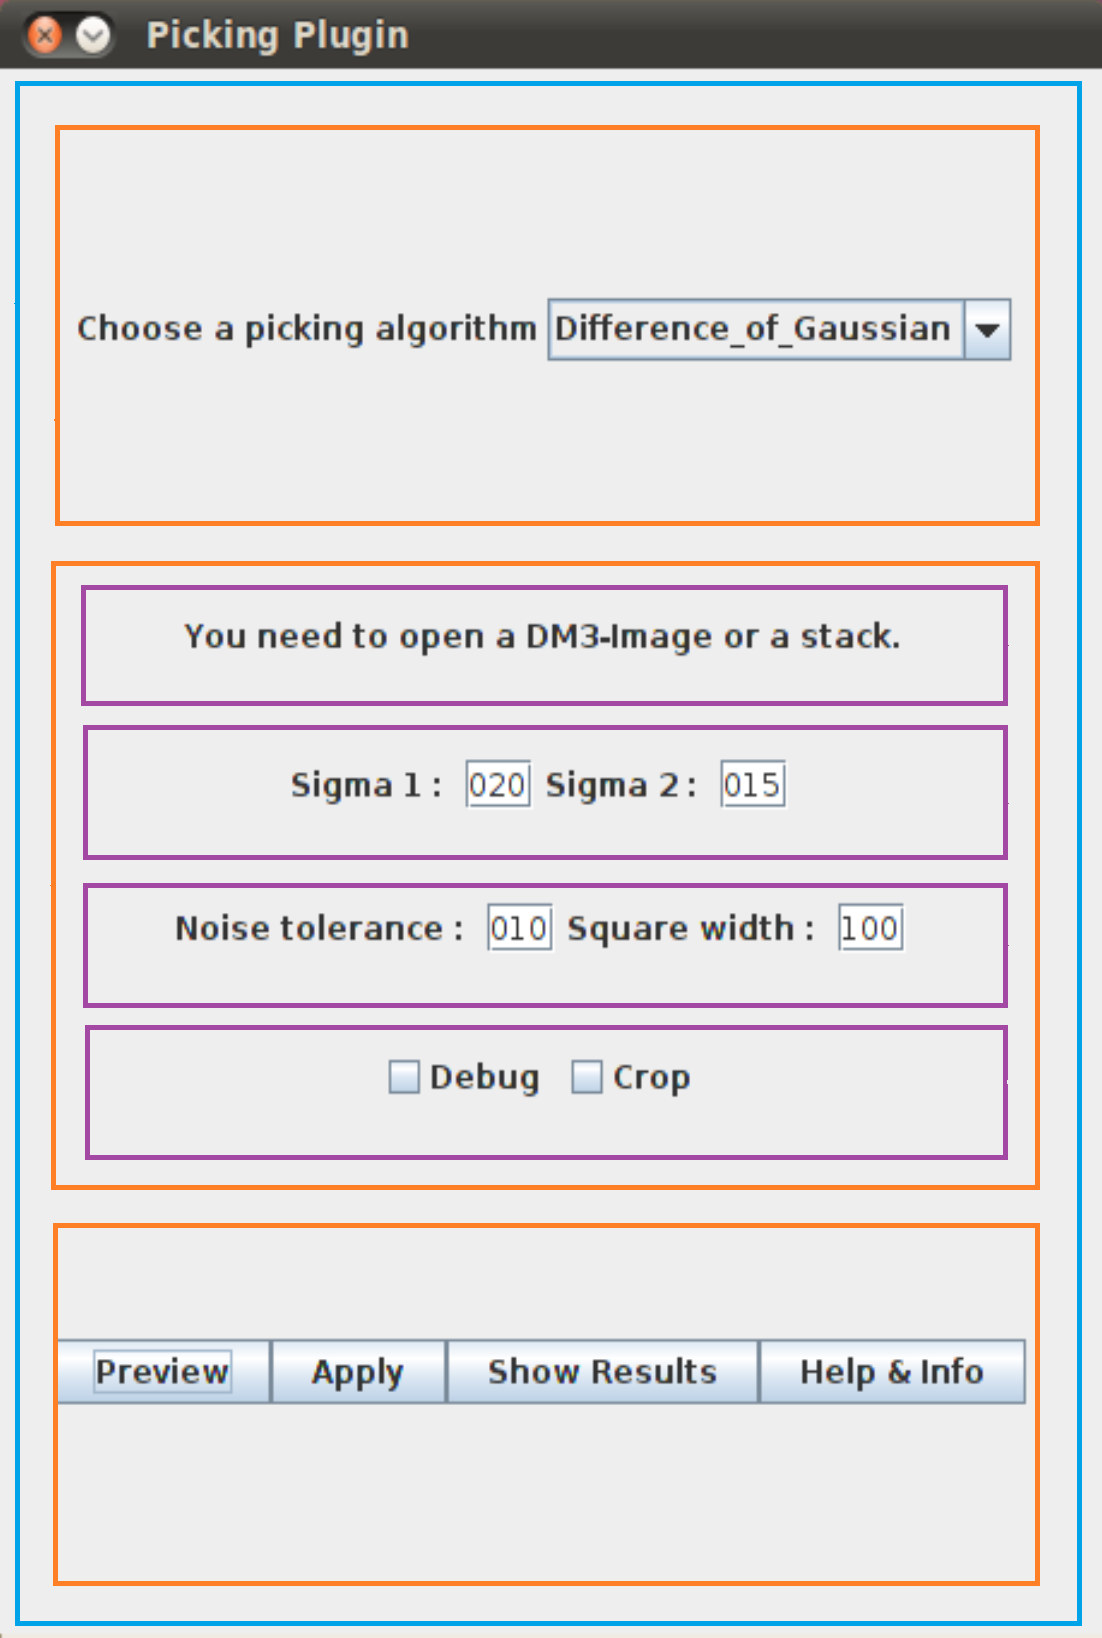
\includegraphics[width=0.4\textwidth]{pluginCadres.png}
\caption{Organisation des panels pour l'algorithme Difference of Gaussian}
\label{panneaux}
\end{center}
\end{figure}
\pagebreak

\subsection{Boutons}

Les boutons doivent répondre aux clics de la souris et lancer l'action correspondante en fonction de l'algorithme de piquage choisi par l'utilisateur :

\begin{description}
\item \textbf{Le bouton de prévisualisation} permet de tester le piquage obtenu par l'algorithme sélectionné sur l'image courante.
\item \textbf{Le bouton d'exécution} permet d'appliquer l'algorithme sur l'image ou le stack sélectionné, lorsque l'utilisateur est s\^ur des paramètres qu'il souhaite appliquer.
\item \textbf{Le bouton d'information/aide} est une aide d'utilisation du plugin ainsi que des conditions de fonctionnement des algorithmes.
\item \textbf{Le bouton d'affichage des résultats} permet d'afficher et de sauvegarder le tableau des coordonnées des particules sélectionnées.% avec l'aide d'\imj.  
\end{description}
Pour que le plugin puisse fonctionner, l'utilisateur devra au préalable avoir ouvert une image ou un stack d'images à l'aide d'\imj.
\pagebreak

\section{Récupération des paramètres}

Les méthodes de piquage ont une classe mère commune. L'utilisateur sélectionne un algorithme dans le menu déroulant et détermine certains paramètres. Quelques uns sont propres aux algorithmes et d'autres sont communs à tous tel que :
%Lorsque l'utilisateur sélectionne un algorithme dans le menu déroulant, il doit choisir plusieurs paramètres.

\begin{itemize}
\item la gestion du bruit de fond,
\item la taille des images des particules sélectionnées lorsqu'on demande le stack d'images,
\item l'activation du débogage (s'il est implémenté dans l'algorithme),
\item l'activation du découpage des particules à partir du piquage obtenu.
\end{itemize}

\section{Algorithmes}

\subsection{Corrélation d'image}

Le principe de cette méthode est de corréler une image de cercle d'une taille définie avec notre image de base, convertie en image binaire. Pour chaque pixel noir on trace un cercle ayant ce pixel pour centre.
Si le cercle est de la m\^eme taille que la particule, les cercles se croiseront tous au centre de celle-ci, formant un point blanc central. Nous obtenons donc une image résultante de corrélation présentant des maxima blancs au centre de chaque particule, dont la taille est identique à celle du cercle.\\
Cet algorithme trouve donc les valeurs élevées de pixel correspondant à la meilleure superposition locale entre l'image de référence (le cercle) et l'image de base.\\

%Le principe de cette méthode est de comparer une image contenant un cercle avec l'image sur laquelle on veut sélectionner les particules. On obtient alors une nouvelle image sur laquelle on peut voir des cercles correspondant aux particules de l'image de base qui ont à peu près le même diamètre que le cercle dessiné précédemment. Ici, on fait varier la taille du cercle afin de sélectionner des particules de différentes tailles.\\
\noindent
Pour cette méthode de piquage, l'utilisateur doit entrer le rayon minimal et maximal des particules à sélectionner, ainsi que la valeur de l'incrémentation.\\ Pour un résultat optimal, avant de lancer la sélection des particules avec cet algorithme, l'utilisateur devra traiter l'image pour éliminer un maximum de bruit de fond (utilisation de filtres).

\subsection{Différence gaussienne}

La différence de Gauss est une technique qui soustrait une image à laquelle à été appliqué un filtre gaussien à une deuxième image possédant une valeur d'écart-type plus petite, donc moins filtrée. Par conséquent, les bords des particules sont dégradés, nous permettant de récupérer les maxima de l'image résultante, c'est-à-dire le centre des particules.\\
%La différence de Gauss est une technique qui consiste en la soustraction d'une version floutée %de l'image d'origine à une autre version moins floutée de cette même image.\\
\noindent
Il est demandé à l'utilisateur d'entrer les valeurs d'écart-type qui seront utilisées pour appliquer les filtres gaussiens.

\subsection{Différence de dilatation}

Cette méthode repose sur le même principe que la différence gaussienne, à ceci près que l'image d'origine n'est pas floutée. Nous lui appliquons un certain nombre de cycles de dilatation et obtenons alors des particules de plus grandes tailles. A la soustraction des deux images, seuls les contours des particules apparaîtront, nous permettant de récupérer le centre de particules.\\
L'utilisateur devra entrer les nombres de cycles de dilatation qu'il souhaite appliquer à chaque image.

\section{Stack d'images résultantes}

Si l'utilisateur le désire, il peut récupérer un stack contenant les particules piquées. Ce stack est obtenu à partir du tableau des coordonnées que la fonction de création du stack prend en paramètre d'entrée.
Les particules trop près du bord sont éliminées, les autres ajoutées dans un stack qui est finalement affiché à l'utilisateur.

\section{Organisation orientée objet du programme}

Afin de clarifier et de simplifier le code, nous avons tenté de séparer les grandes fonctions du programme en suivant les principes de la programmation orientée objet.

\subsection{Séparation interface graphique et traitement d'images}

Sans suivre le patron de conception Modèle-Vue-Controleur (MVC), nous avons créé différentes classes permettant de distinguer la partie GUI de la partie algorithme. Nous obtenons ainsi des classes ne gérant que l'aspect graphique du plugin. Celles-ci gèrent plus particulièrement les panneaux propres aux méthodes de piquage ainsi que les classes bien distinctes effectuant les traitements d'images.

\subsection{Séparation traitement d'images et création du stack}

La partie permettant la création du stack d'imagettes à été séparé des méthodes de piquages afin d'éviter la répétition de ce code dans chaque algorithme. Cela permet aussi d'y faire appel en dehors de nos algorithmes contrairement à une implémentation de cette fonction dans une classe mère.

\subsection{Patrons de conception}

Cette séparation GUI/traitement/stack à dû être accompagnée de la création de classes suivant des patrons de conception particulier : la \emph{factory} et le \emph{singleton}. 
\begin{description}
\item[La \emph{factory}] permet d'instancier des objets dont le type est dérivé d'un type abstrait. La classe exacte de l'objet n'est donc pas connue par l'appelant. La classe en \emph{factory} rend possible les transitions entre chaque méthode de piquage. Elle amorce le panneau propre à l'algorithme permettant d'actualiser l'interface et ainsi de récupérer les paramètres utilisateur. Ensuite, lorsque l'utilisateur clique sur les boutons d'exécution ou de prévisualisation, la \emph{factory} lancera les actions correspondantes.
\item [Le \emph{singleton}] est un patron de conception (design pattern) permettant de restreindre l'instanciation d'une classe à un seul objet (ou bien à quelques objets seulement). La classe en \emph{singleton} permet de conserver les paramètres choisis par l'utilisateur. De ce fait, même lorsqu'il exécute plusieurs algorithmes, une seule instance de cette classe peut exister, actualisant les paramètres choisis par l'utilisateur.
\end{description}


\subsection{Modularité et réutilisation du code}

L'organisation orientée objet du code a fortement facilité l'écriture du programme, évitant la répétition de lignes de code qui pouvaient \^etre factorisées. De plus, cela permet une grande modularité au sein de notre programme, facilitant l'ajout ou le retrait d'un algorithme de piquage et de son interface dans notre plugin. Cette modularité est telle qu'elle permet, en ce qui concerne le module de création du stack de particules sélectionnées, de l'utiliser en dehors de notre plugin.\\
Cela tient un rôle important dans notre projet car, comme pour beaucoup de logiciels libres, \imj ~se développe beaucoup gr\^ace à sa communauté d'utilisateurs qui participe au développement de plugins. Après validation par le personnel du NIH \footnote{National Institute of Health} responsable de ce projet, les plugins sont mis à la disposition des utilisateurs. Ainsi, chacun pourrait ajouter/améliorer des méthodes de piquage de particules, développant et augmentant l'efficacité et la sélectivité de notre plugin. \\

Ci-après (Figure \ref{classes}) le diagramme général de l'organisation de nos classes :

\begin{figure}[!h] 
\begin{center}
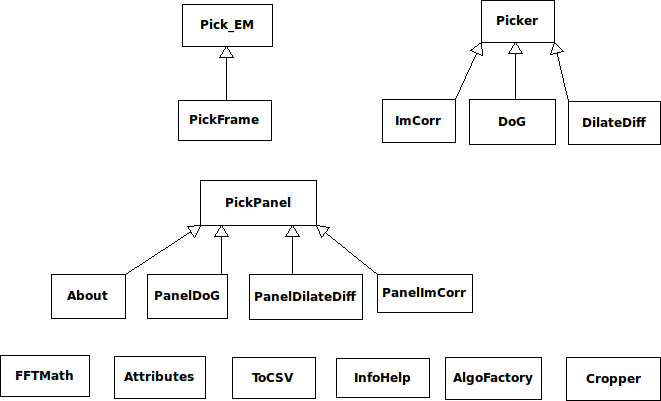
\includegraphics[width=0.8\textwidth]{class_diagram.png}
\caption{Organisation générale des classes du plugin Pick\_EM}
\label{classes}
\end{center}
\end{figure}


%\section{Les classes}
%
%Le programme est divisé en seize classes distinctes:
%\begin{list}{

%\item Une première partie regroupe six classes qui permettent de gérer l'interface graphique.
%\item
%\item Une seconde partie regroupe les algorithmes de piquage, elle est composée de quatre classes.
%\item La classe \texttt{AlgoFactory} sert de pivot au programme en fonction du choix d'algorithme de l'utilisateur (adaptation de l'interface et algorithme de piquage).
%\item La classe \texttt{Attributes} est un singleton (instanciable qu'une seule et unique fois) et contient tous les paramètres à entrer par l'utilisateur pour faire fonctionner les algorithmes.
%\item La classe \texttt{Cropper} est une fonction subsidiaire du piquage permettant de créer un stack dans lequel chaque image contient une particule piquée (si l'utilisateur le demande).
%\item La classe \texttt{FFTMath} contient la méthode permettant de faire la Corrélation d'images.
%\item Les classes \texttt{About} et \texttt{InfoHelp} contiennent des informations et une aide sur l'utilisation du plugin.
%\end{list}
%
%\subsection{Les classes de l'interfaces}
%
%La classe \texttt{Pick\_EM} fait le lien entre \imj ~et la classe \texttt{PickFrame} qui est une JFrame, elle permet de créer l'interface graphique.\\
%Vient ensuite la classe \texttt{PickPanel} qui permet d'adapter l'interface en fonction de l'algorithme. En découlent \texttt{PanelDilateDiff}, \texttt{PanelDoG} et \texttt{PanelImCorr} pour leurs algorithmes respectifs (Dilate Difference, Difference Of Gaussian et Image Correlation).
%
%\subsection{Les classes des algorithmes}
%
%La classe \texttt{Picker} est utilisée pour appeler les algorithmes. Les algorithmes étant \texttt{DialteDiff}, \texttt{DoG} et \texttt{ImCorr}.
%Pour faire fonctionner ces algorithmes, la classe \texttt{Attributes} renvoie les valeurs des paramètres entrés par l'utilisateur.
